\chapter*{Rules - Examples - Tests}

\ifnotes
    Point out that there are 2 pages associated with this concept centre. Explain that the first one (the diagram) is the most important, so if they don't get through the second exercise , not to worry.
    
    Learning outcomes:
    
    \begin{itemize}
        \item Explain that Rules = requirements = acceptance criteria
        \item Annotate arrows in diagram: illustrate, can become, verify
        \item Describe how examples form the foundation of unambiguous shared understanding
    \end{itemize}
    
    Ask the delegates for the labels they came up with. If possible, respond with "yes, and...". Have 3 index cards/stickies ready with the labels you want to use. [Don't write on the posters - dry wipe doesn't come off the laminate!]
    
    Now make sure that they've noticed that concrete examples can help share knowledge. They give the person that comes up with them a way to ask, "Should the system behave like this?" and the expert the chance to say "Yes", "No", or "I don't know".
\fi

\ifcontent

    \QandAbox{Rules, Examples, Tests - how are they related?}{2.5}
    
    Having discussed the relationships between Rules, Examples and Tests try and come up with a word (or short phrase) that describes each of the relationships represented by the arrows in the diagram. 
    
    \underline{\textbf{Write them in your workbook, on the diagram below}}:
    
    \vspace{2cm}
    
    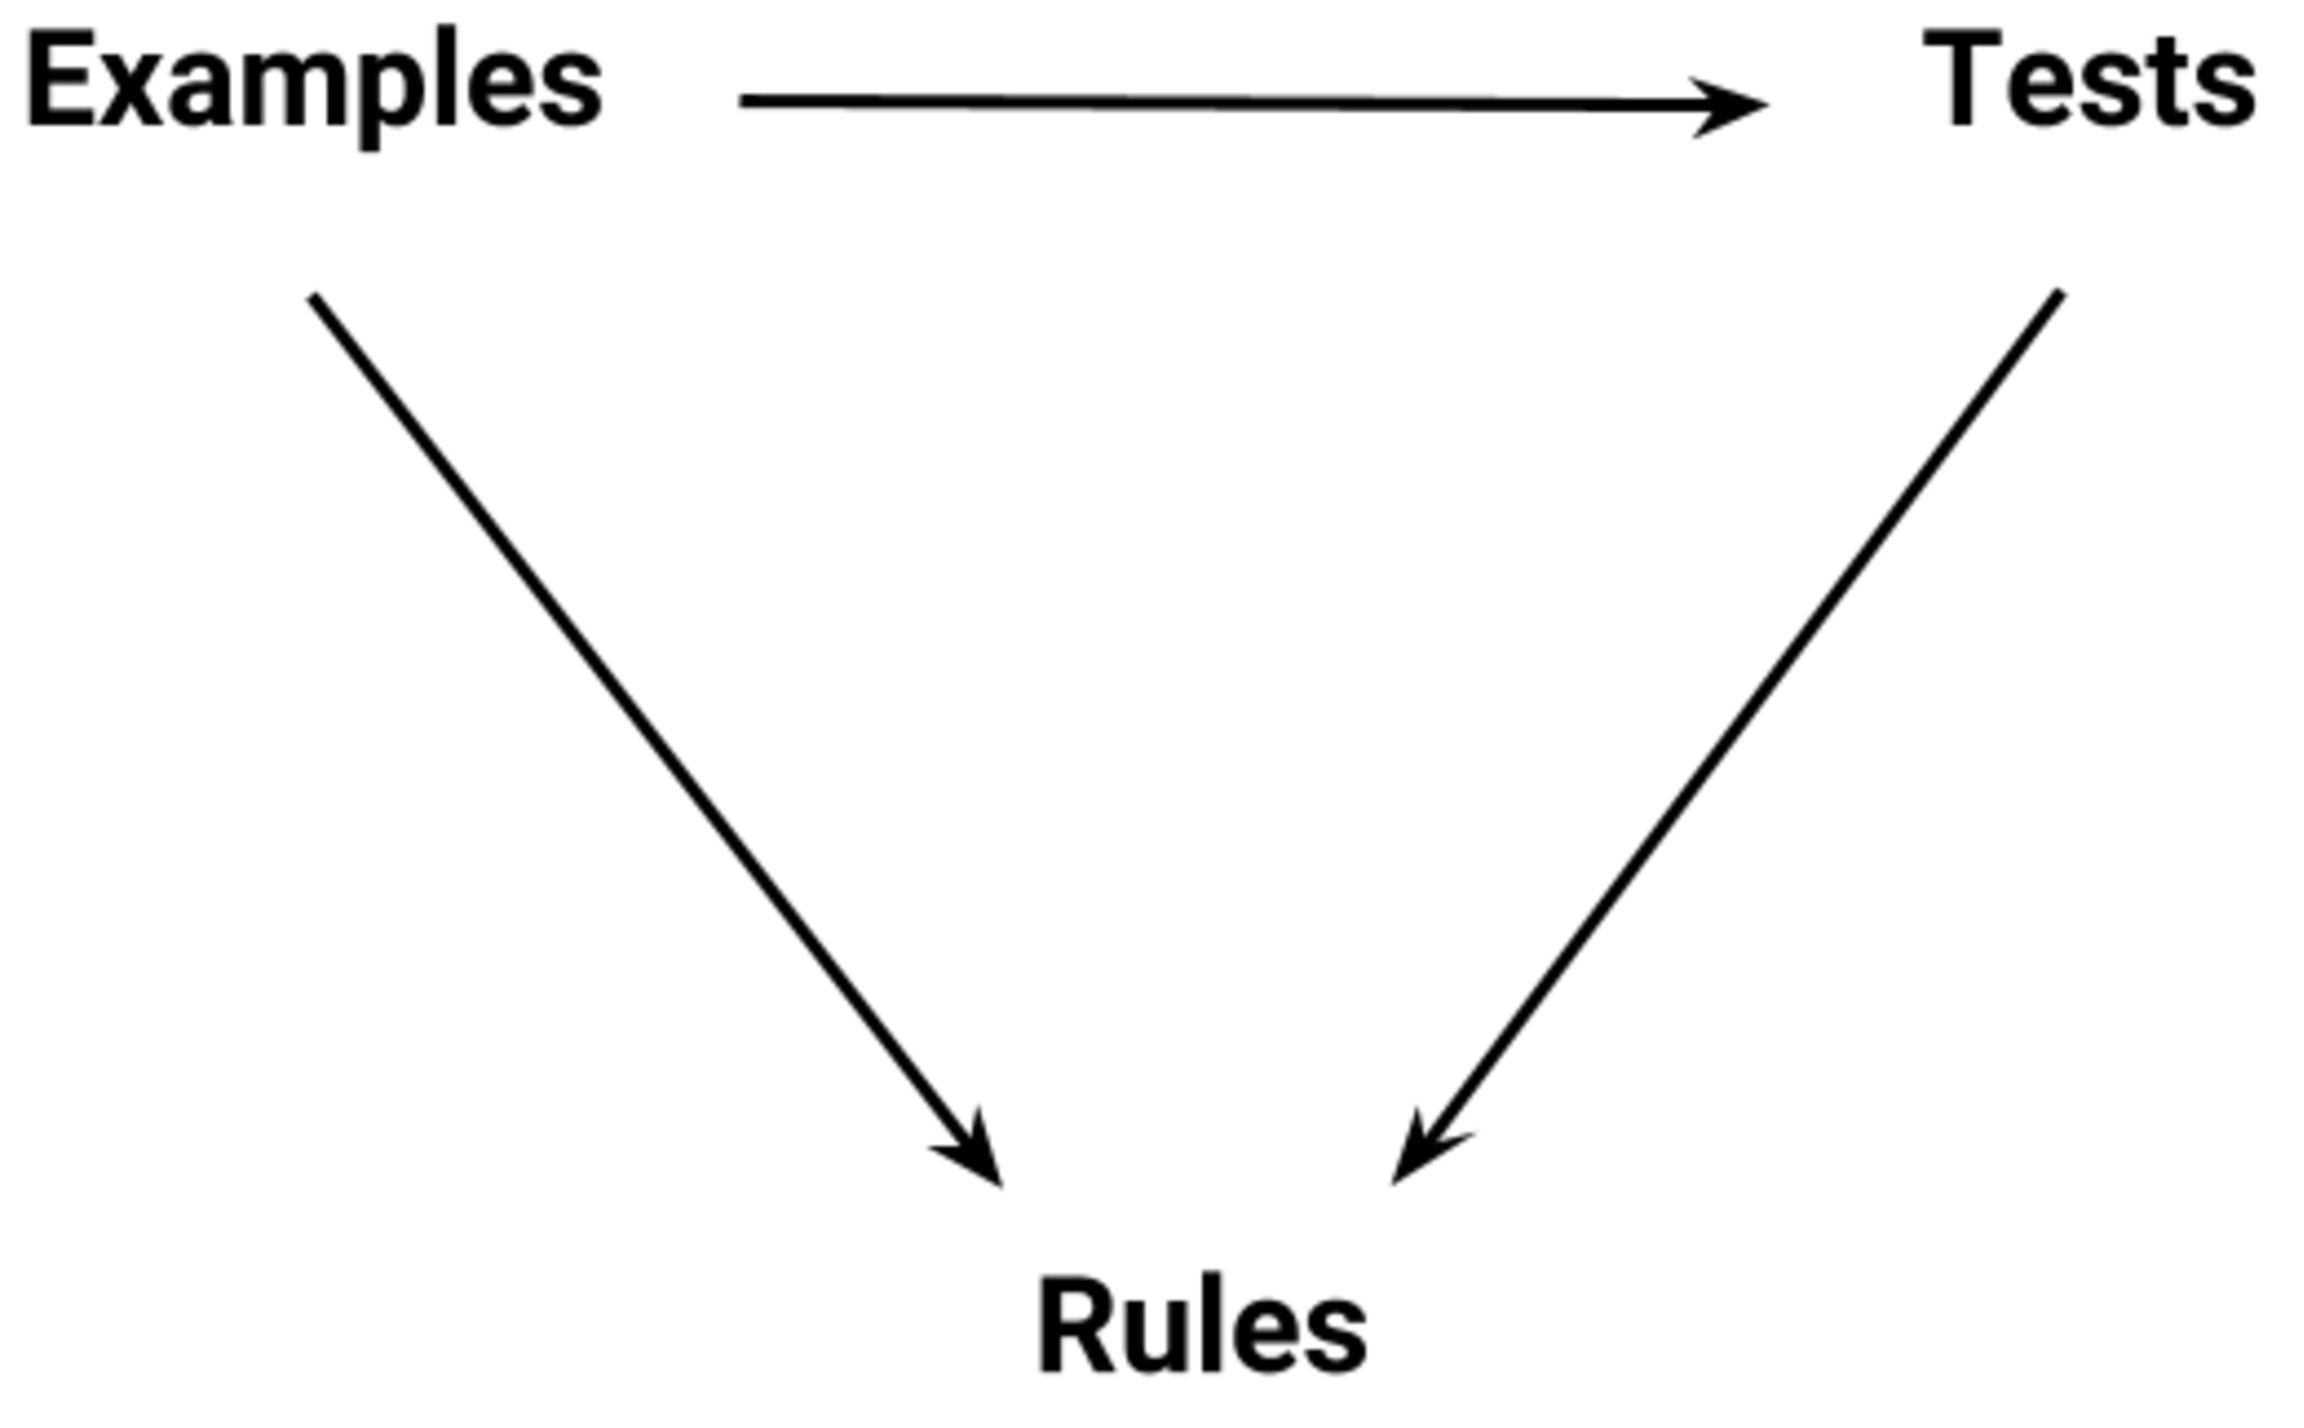
\includegraphics[width=\textwidth]{images/examples-tests-rules}
\fi


\chapter*{Rule or example?}

\ifnotes
    Learning outcomes:
    
    \begin{itemize}
        \item Describe why, when taken individually, it can be hard to decide whether a statement is a rule or an example
        \item Explain what a rough example is and why they shouldn't be used
    \end{itemize}
    
    You can review this exercise by asking delegates to "channel their inner 3-year old". You read out the number, and they all respond with a chorus of "Rule" or "Example". If they all get the "right" answer, then you move on to the next. If they get different answers, then stop to discuss why.
    
    "The one where the customer forgot their credit card" is called a rough example - described in Introducing Example Mapping. Tell the class that it's better to consider this a Bad or Incomplete Example. Don't use this format of example in the class. Avoid using them in real life.
    
    "When an avid reader buys four books in one month, the cheapest of the four should be free" - is this a rule? It could be an example illustrating a more general rule - without the context it's impossible to say.

\fi

\ifcontent
    Consider each of the statements below. Is it a rule or an example? Write an “R” if you think it's a rule, and an “E” if you think it's an example. When you're done, swap with someone on your table and mark each other's answers. If there is any disagreement - discuss!
    
    \begin{enumerate}
        \item People logging on for the first time should be shown a summary of their team's activity.
        \item A loan of \$10,000 with 5\% annual interest, repaid at \$100 per month should have a balance of \$9,140 after 13 months.
        \item Sally is standing in Times Square, and Jimmy is at a Starbucks 50 feet away with the app open. When Sally shouts "Can anyone hear me", Jimmy receives the shout on his smartphone.
        \item The total charge for the customer's basket should include all applicable discounts.
        \item A purchase of wine for \$20 and beer for \$5 with a 10\% discount coupon gives a checkout total of \$22.50
        \item Always log off the user when their session has been inactive for the timeout period
        \item The one where the customer forgot their credit card
        \item When an avid reader buys four books in one month, the cheapest of the four should be free.
        \item Marketing should be able to create new discount codes without programmer help
        \item A customer buys three books costing more than \$10 each last Tuesday. When they put a \$10 book in their shopping cart today, an "avid reader" discount of \$10 should be presented
        \item If Tom Jones hasn't conducted any transactions since May 1986, then a report of inactive accounts should include Tom Jones's account
    \end{enumerate}
\fi
